\documentclass{article}
\usepackage[utf8]{inputenc}
\usepackage[margin=1in]{geometry}
\usepackage{amsmath, amsthm, enumerate, mdframed, bbm, enumitem, graphicx, titling}
\setlength{\droptitle}{-5em}

\title{Project Final Report: Catan}
\author{Derek Feriancek, Jackson Stogel, Lindsay Yang, Yi Zhao}
\date{}

\begin{document}
\maketitle

\section*{How to run:}

A C extension we have written for computing hitting time is included in the submitted files. Please read the \verb|README.md| for installation details.

\section*{Overview}

We divide our general strategy into two segments. The immediate, greedy strategy, and the overall, long term meta strategy. The goal of our greedy strategy is simply to determine what to do next (how to achieve the next victory point, whether or not to trade, whether or not to build on a given turn). The goal of our meta strategy is to determine what our long term goals are (what goal should we prioritize at this given time, where should we build our settlement, etc).

\subsection*{Definitions}

\begin{itemize}
    \item Goals: sequences of actions that will yield a victory point. There are three types of goals: development card, build city and build settlement. Each goal consists of Tasks.
    \item Tasks: immediate objectives that our AI hopes to achieve. Each task also handles trading to try to achieve the objective. There are four types of tasks: building roads, buying development cards, building a city and building a settlement.
    \begin{itemize}
        \item The dev card goal and the build city goal only consists of one task. However the build settlement goal consists of build road tasks and a build settlement task.
    \end{itemize}
\end{itemize}

\section*{Greedy Strategy}

As stated above, the objective of the greedy strategy is to \textbf{figure out which goal to pursue at the current time}. \\ \\
We stuck with the main idea outlined in our original write up, in which we calculate hitting times to various goals. However, the current optimal goal to pursue is based on this hitting time combined with a special weight function. These weight functions are determined by the meta strategy.  \\ \\
A basic outline of the greedy algorithm is this:
\begin{enumerate}
    \item Calculating the hitting time to all feasible goals 
    \item Pick the best goal with a weight function that takes into account the hitting time
    \item Execute the first task within the best goal
    \item Repeat
\end{enumerate}

\subsection*{Calculating Hitting Times}

After creating a probability transition matrix, we used NumPy’s linalg library to solve for the hitting times. We used a matrix formulation of the hitting time equations: 
$$
(P - I)\beta + 1 = 0
$$ 
To enforce that any given state i (where i is an encoded version of our current resources) was an end state and should have a hitting time of zero, we simply removed column and row i from our transition matrix. 

\subsection*{Trading}

The main difficulty was how to simulate the possibility to trade resources on hand. In order to account for trading, we created a generic trade rule for each task. The trade rule is pretty simple: if we have 4 (or 3 or 2 given a port) extra of a resource, a trade is made to the resource that we’re most deficient in for a given task (i.e. build a road). This is crucial for boards with few of one resource. This trade rule is taken into account when we calculate the hitting time to goals.

\section*{Meta Strategy}

The meta strategy consists of the weight functions which the greedy strategy uses to determine what goal to pursue next. The weights should not only take into account the immediate hitting times to achieve a goal but also the long term investment of achieving more goals at a faster pace in the rest of the game.

\subsection*{Weights functions}

In order to capture the both short term and long term benefits of completing a goal, we designed our weight functions with the following features in mind:

\begin{enumerate}
    \item Hitting time: how fast we can complete the goal given our current resource intake
    \item Prosperity: the increase in resource generation that this goal provides
    \item Current victory points: we adjust our strategy depending on how close we are to finishing the game
\end{enumerate}

\subsection*{Measuring Prosperity}

We measured the long term investment value of a goal by calculating the hitting time to get $\geq 2$ of each resource given that said goal was completed.  This succinct idea combines two important concepts for a good settlement/city/port: it values resources that are placed on high probability squares (6, 7, 8) as well as a diversity of resources in the surrounding squares. The fastest time to hit (2, 2, 2) will need to have a balanced combination of both. As we aren’t fully sure exactly what our future strategy will entail, we thought something that satisfied both properties would give us our best investment toward the future.

\subsection*{Implementation}

We designed our final weight function with softened inverse functions to represent hitting time and prosperity as we are taking the max of the weights. We also wanted to model the diminishing importance of prosperity as we accrued more and more victory points. At 9 victory points, prosperity -> 0 as future investment is pointless. Our implementation is below.

\begin{verbatim}
speed = (1 / (0.1 + hitting_time))
prosperity = (1 - (victory_points / 9.0)) / (0.1 + time_to_gain_resource)
return h1 * speed + h2 * speed * prosperity + h3 * prosperity
\end{verbatim}
Here, h1, h2, h3 are our hyperparameters. We set our final hyperparameters through naive search.

\section*{Optimization}

In order to reduce our computation time, we made extensive use of caching results and also wrote a C extension for python to handle building the transition matrix. All of our trading functions and hitting time results are stored in LRU caches as our approach calls each of these functions repeatedly: approximately 70\% of our hitting time and trade decisions functions are repeated calls. However, this optimization alone was not enough. \\ \\
The slowest part of our program was the transition matrix generation code, since Python for-loops can be quite slow. In order to create this matrix as fast as possible, we wrote a simple C extension for python that generates this transition matrix as a NumPy array. After optimization, one hundred simulations (which contains ~20,000 non-cached hitting time calculations) ran in around 12 seconds on our machine. \\ \\
While this worked quite well, we would have liked a pure NumPy solution, as it is much simpler. However, none of us knew how to perform NumPy wizardry for vectorization or were sure it was even possible in this case due to trade rules.


\section*{Performance}

We had a \textbf{mean performance of 58.2} turns on ten randomly generated boards run 100 times each. The following histogram is unnecessary but pretty. It shows the runtimes over 10,000 distinct boards each simulated once.

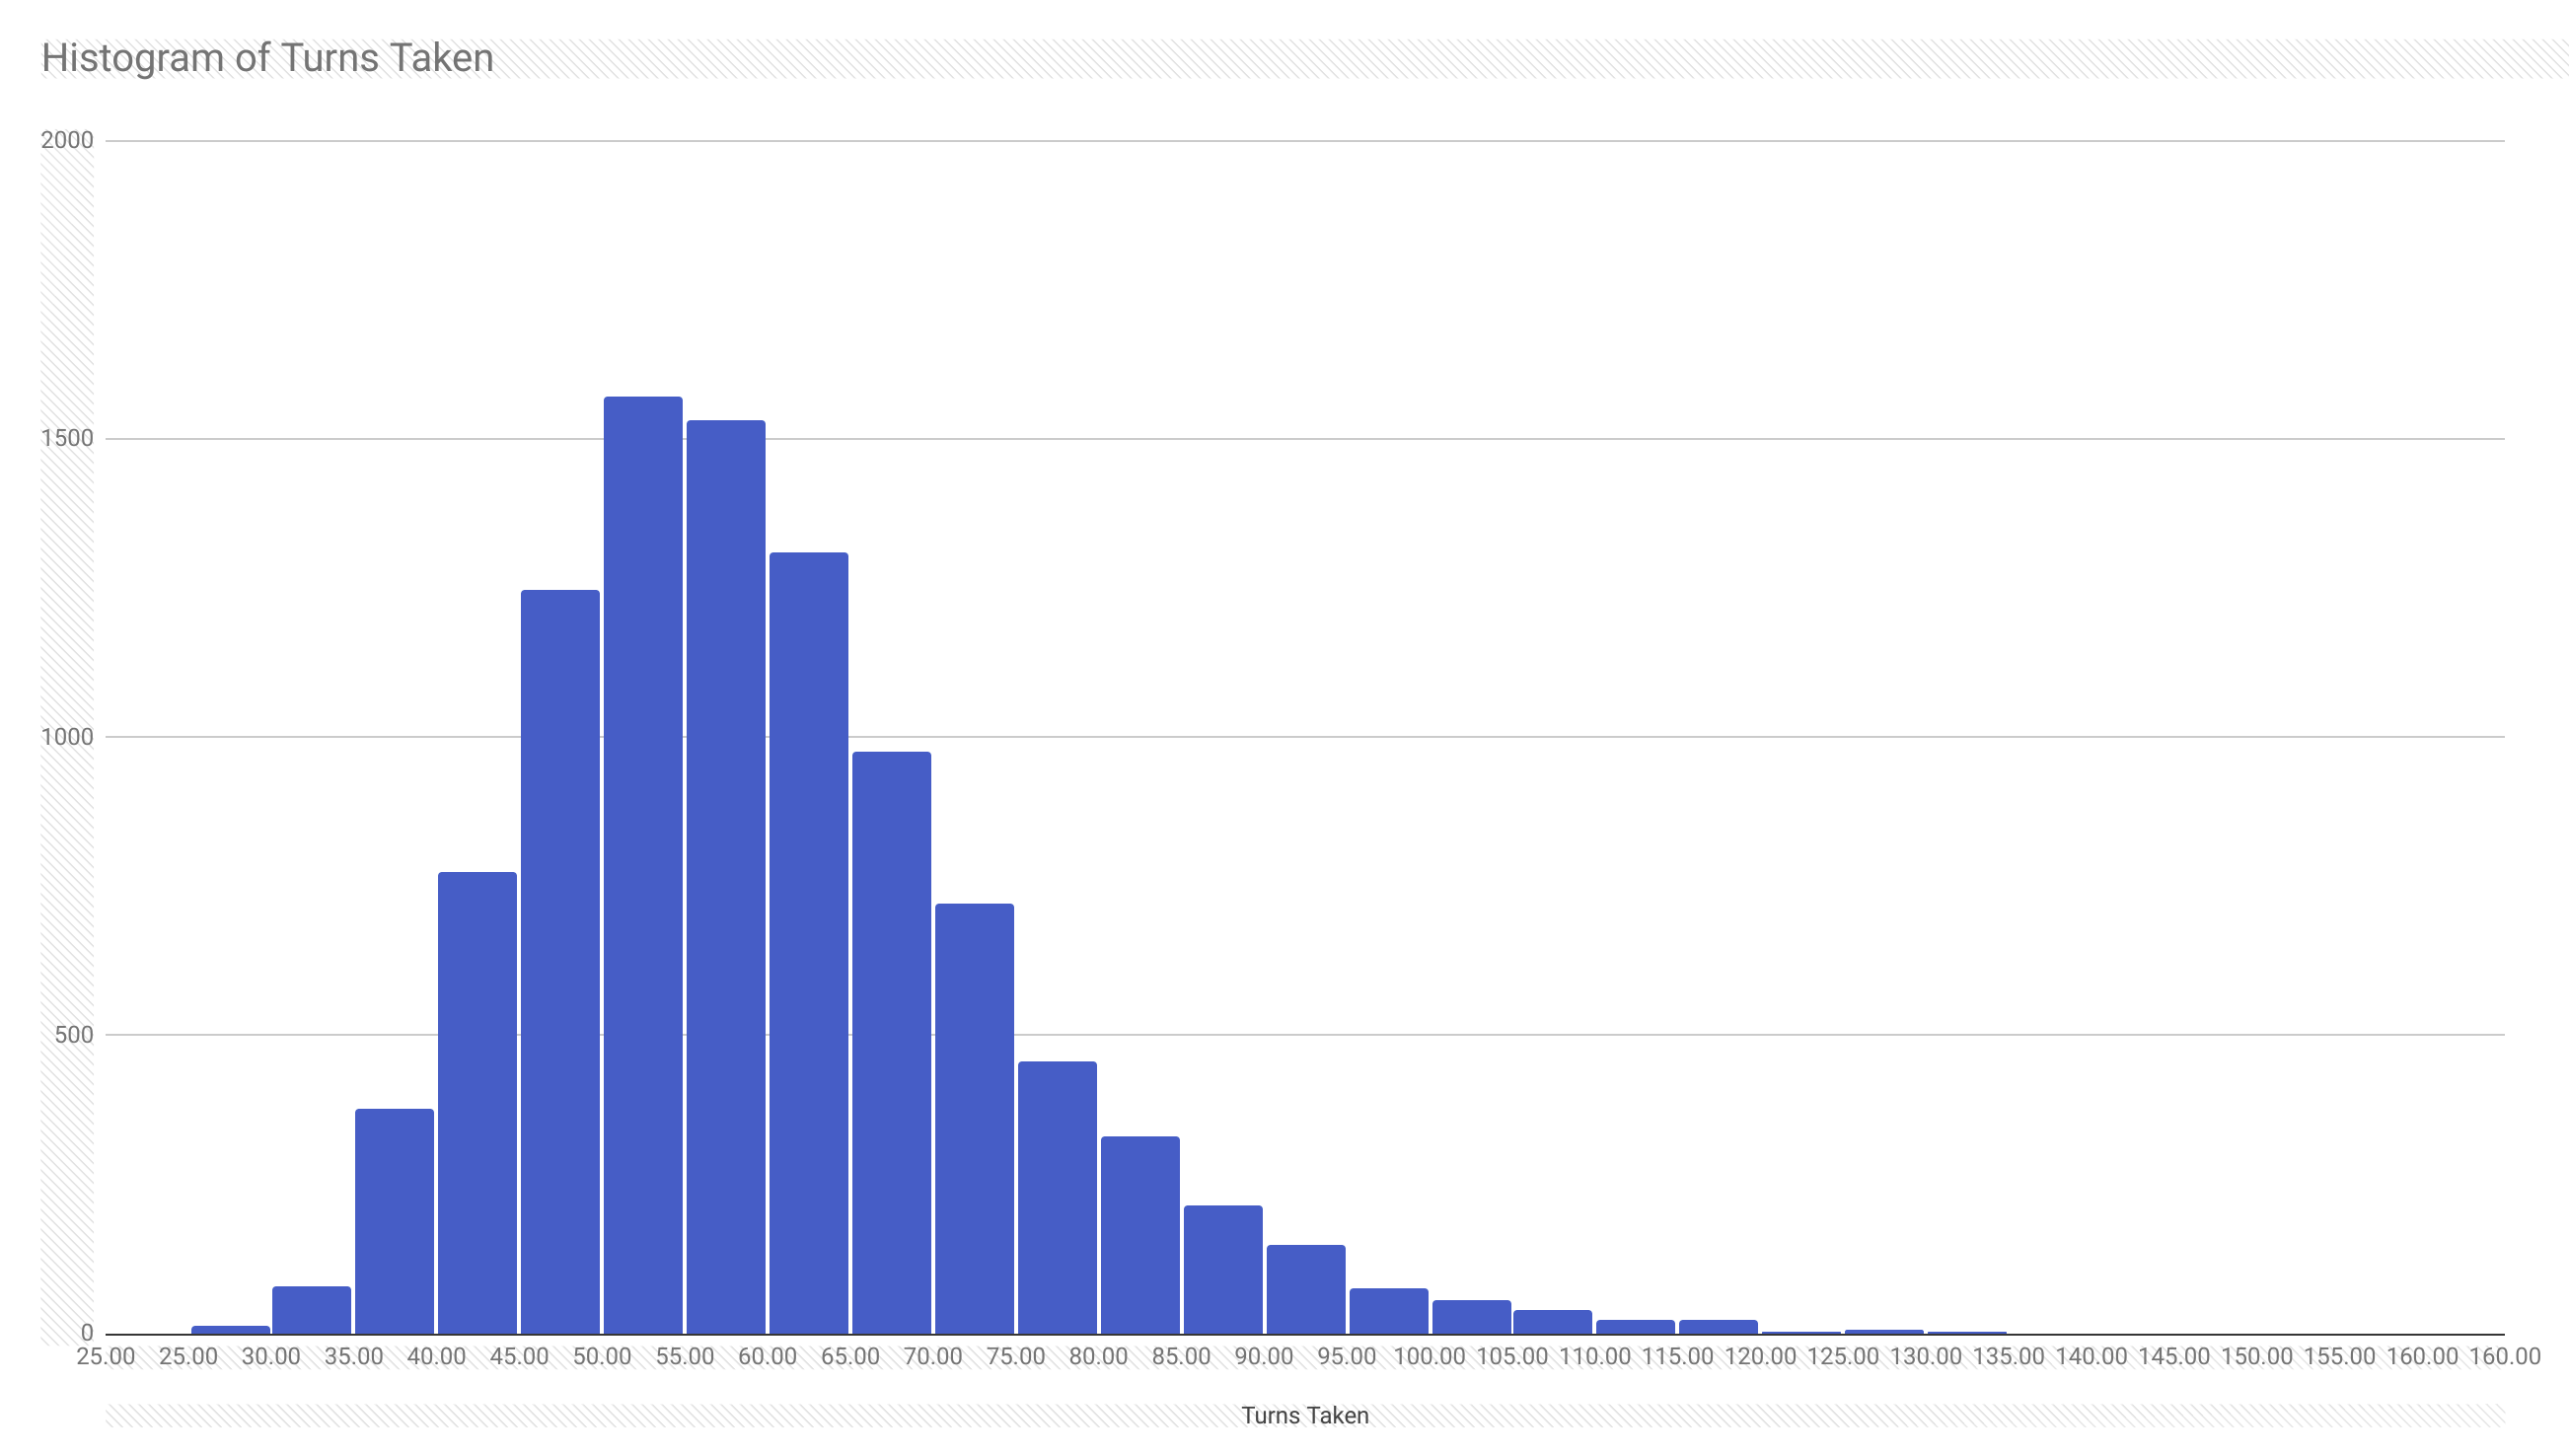
\includegraphics[scale=.18]{histogram.png}

\section*{Scrapped Ideas and Improvements}

\subsection*{Initial Brainstorm}

Originally, we tried to simplify hitting time calculations by using an “average resources gained per turn” heuristic, in which we calculate that for any given configuration (ie settlement/road/city configuration), we try to figure out how many resources we can gain averaged over all dice rolls and their respective probabilities. However, we quickly realized this would be a great oversimplification for calculating hitting times, but might be better for a weighting function later on for calculating objective to pursue. We wanted to recompute hitting times upon reaching a new configuration, but this does not take into account resource gain each turn enough. \\ \\
For every possible objective, we calculate the hitting time and then select the minimum, which remains a general strategy throughout the entire project. At this stage of brainstorming, we simplified trading into trading any resources that was $> 4$ into the resource we had the least of. 


\subsection*{Improvements}

Our meta strategy could still be improved. If we had additional time, we would have experimented with more models and tested hyperparameters more thoroughly. One feature that we didn’t consider is the closeness of potential settlements to ports. This could be valuable if a board is extremely deficient in a potential resource and extremely plentiful in another.

\end{document}
